\hypertarget{group__CNC}{\section{C\-N\-C}
\label{group__CNC}\index{C\-N\-C@{C\-N\-C}}
}


Comand and control tools for system managment.  


Collaboration diagram for C\-N\-C\-:
\nopagebreak
\begin{figure}[H]
\begin{center}
\leavevmode
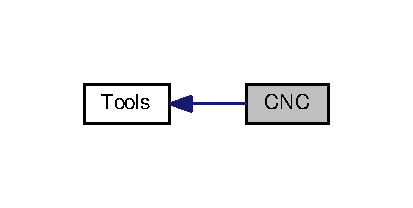
\includegraphics[width=198pt]{group__CNC}
\end{center}
\end{figure}
Comand and control tools for system managment. \hypertarget{group__CNC_IPMITool}{}\subsection{I\-P\-M\-I\-Tool}\label{group__CNC_IPMITool}

\begin{DoxyParams}{Parameters}
{\em target} & List of remote host names or L\-A\-N interfaces to monitor during reset operations \\
\hline
{\em controller} & List of I\-P addresses of remote node controllers/\-B\-M\-Cs \\
\hline
{\em username} & Remote session username \\
\hline
{\em password} & Remote session password \\
\hline
{\em pwfile} & File containing remote session password \\
\hline
{\em command} & Command to be sent \\
\hline
{\em maxtries} & Max number of times to ping each host before declaring reset to fail \\
\hline
{\em numthreads} & Number of worker threads to use \\
\hline
{\em dryrun} & Dryrun -\/ print out commands but do not execute \\
\hline
{\em sudo} & Use sudo to exeute privilaged comands \\
\hline
\end{DoxyParams}
